\chapter{Results and Considerations}
In this chapter the results and the material created during all the work of this thesis are discussed.
It is important to highlight that the results are not the only parameter defining whether a good verification work was done or not. In fact, building the infrastructure and create documentation are important tasks that every verification engineer will eventually do. Even if these tasks are not always directly correlated to some found bug, they will produce results in long term.


\section{Found Bugs}
The thesis was developed while the design and the specifications were still in progress and so unstable. To synchronize all the work it was used the GitLab structure, creating issues and discussing the problems. A well defined issue was then assigned to a design engineer to fix it.

The majority of the bugs were found on the Load Management Unit. Let's now analyze some of them.

\subsubsection{Indexed load bug}
This issue was found using the Formal tools and trying to define better specifications for the Load Management Unit.

The problem was the following:
The LMU used the \emph{sequence\+id}, in particular the \emph{el\+count} field, to identify if the load was strided or indexed. In particular, \emph{el\+count} contains the number of valid elements being loaded; when this value was \emph{el\+count = 1} the load was considered as indexed.
The issue was occurring because the indexed load should have ignored the stride value, but this was not the case. In fact, the load would not have ignored the stride, as every operation was actually considered as a strided one.

The best solution for this problem was to create a new signal, \emph{is\+indexed}, to identify an indexed load. The stride will be always ignored when this signal is asserted, and the value of \emph{el\+count} must be equal to 1.

\subsubsection{Load id bug}
This issue regards the load ids. When a load was finished, the \emph{load\+sync\+end\+i} signal was sent to the LMU to notify the operation was concluded.
It was sent without an identifier to understand which of the two possible loads was finished, so a FIFO was used to end them in order.
This was an issue because the loads should have the possibility to end out-of-order, so a new signal was created: \emph{load\+sync\+end\+sb\+id\+i}. This signal is the id that identifies the load to be finished.
This issue was found analyzing the specifications to create the Test Plan.

\subsubsection{Out-of-order load bug}
This issue regards the out-of-order loads. In the Load Management Unit there is a FIFO handling the load ids for the two possible inflight loads.
The FIFO was freed of an element only when another one was put as input. But it could have been happened that an already inflight load was into the FIFO, i.e. with \emph{id = 1}, and another load with the same id, issued.
Having the same id, the configurations for the second load would have been overwritten.

This issue was found analyzing the result of two consecutive loads, with same id, but one was strided and another one was indexed. The second load was not considered as indexed, failing the condition that says that \emph{el\+count = 1}.
This was the case of a typical bug finding flow: first, a big test fails during a load. Then, it is examined using the assertions on the load modules. Exploring the waveform is then possible to find the bug.

\subsubsection{After kill bug}
This bug is related to the validity of the output of the LMU.
When there is a kill, the entire instruction needs to be killed. But, it could be possible to receive valid data for a killed load. This happens because the kill mechanism needs some time to stop the operation.
The LMU should ignore the input from a killed instruction, but it did not happen in this case. Indeed, the validity of the data in output was assumed every time the data was valid in input.
This caused the simulation to timeout on the next instruction. This was happening because the kill was not issued correctly, so the starting point for the next instruction was not clean.

This issue can represent a valid example of why the formality on the assertions in very important.
Consider the following code:


\linespread{1}
\begin{lstlisting}[language=Verilog,style=verilog-style, backgroundcolor=\color{lyel_palette}, frame=tlb]
property p_dvalid_o;
@(posedge clk_i)
load_data_valid_i && sb_correct |-> ##1 load_dvalid_o ;
	endproperty : p_dvalid_o

a_dvalid_o : assert property( disable iff(!rsn_i || kill_i) p_dvalid_o )
else $error('LMU did not compute any output');
\end{lstlisting}
\linespread{1.2}

In this case, the assertion is testing if there is \emph{load\+dvalid\+o} when the input is valid. But it does not test if \emph{load\+dvalid\+o} has always a valid \emph{load\+data\+valid\+i} a clock cycle before.
The property as reported is not able to spot the error in this issue, but knowing where the problem is, it is possible to use the correctness of this assertion to understand the bug.

\subsubsection{Two loads bug}
This issue was spotted both in the LMU and in the LB. The modules received two loads with the same id. This led to an assumption error, as every load has an unique id.
In reality the problem was not in the Load Management Unit nor in the Load Buffer, but in the memory queue. In fact, this modules is the one supposed to hand the ids for each load.
This issue was found very late in the verification process because was depending on a trigger enabled by the kill.

For reference in Figure \ref{2-loads} there is the interface of a simulation, in particular on the waveforms. It is possible to see two loads issue with the same id.

\begin{figure}[H]
    \centering
    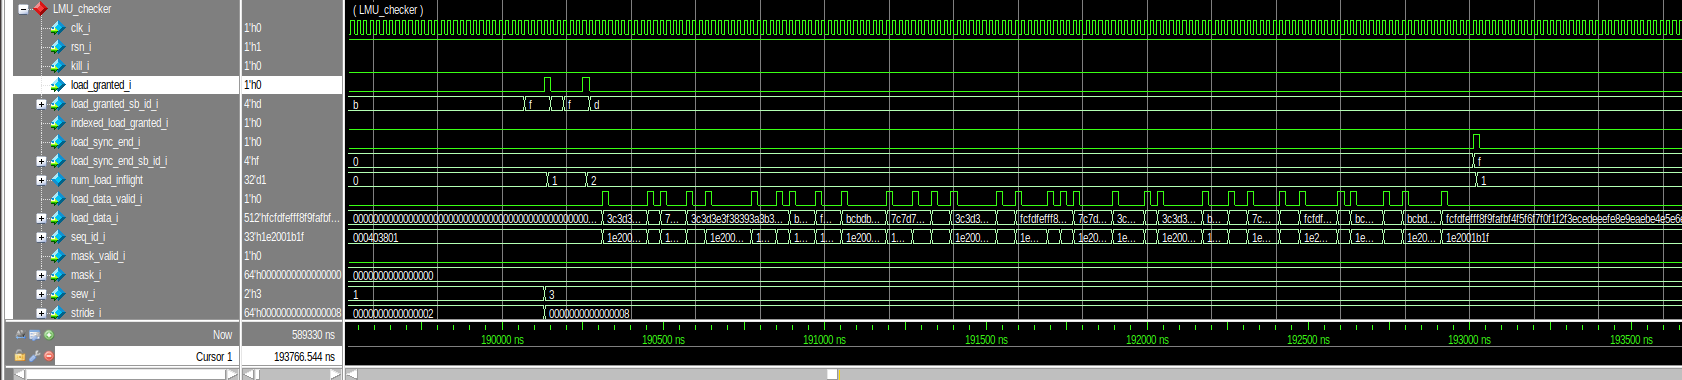
\includegraphics[scale = 0.25]{Chapter_3/img/2-loads.png}
    \caption{Two loads issued with the same id}
    \label{2-loads}
\end{figure}


\section{Material Created}
Beside than the found bugs, during the thesis, some material has been created.
In particular regarding the structure to handle the test of the submodules.

\subsubsection{UVM}
A complete UVM was created, to drive and test the Load Management Unit. It may have different tests with different sequences and so different constraints.

\linespread{1}
\begin{lstlisting}[language=Verilog,style=verilog-style, backgroundcolor=\color{lyel_palette}, frame=tlb]
class lmu_constrained_test extends lmu_random_test;
    `uvm_component_utils(load_management_unit_constrained_test)

	function void build_phase(uvm_phase phase);
		lmu_sequence_item::type_id::
		  set_type_override(lmu_constrained_sequence_item::get_type());
		super.build_phase(phase);
	endfunction

	function new(string name, uvm_component parent);
      		super.new(name,parent);
   	endfunction : new


endclass : lmu_constrained_test
\end{lstlisting}
\linespread{1.2}
In this code the base\+test is extended and then it is overridden into the build\+phase the sequence\+item.


\linespread{1}
\begin{lstlisting}[language=Verilog,style=verilog-style, backgroundcolor=\color{lyel_palette}, frame=tlb]
class lmu_constrained_sequence_item extends lmu_sequence_item;
	`uvm_object_utils(lmu_constrained_sequence_item)

	constraint few_rst{op dist{rsn_op:=1,gnt_op:=5,load_op:=9,kill_op:=2};}
	
	function new(string name = "");
		super.new(name);
	endfunction : new

endclass : lmu_constrained_sequence_item
\end{lstlisting}
\linespread{1.2}
In the sequence new constraints are applied. In this case the probability for the operation are defined.
This kind of structure is very reusable and expandable, furthermore, during the whole verification process it can be improved.

\subsubsection{Specifications}
Some documentation was created on missing specifications.
This work required a looped check on the behaviour obtained by the RTL design. The specifications and the design were still being developed, this does also mean that the documentation should have been updated. But this was not always the case, so a constant check (helped by the formal tool) helped in maintaining the documentation correct.

\subsubsection{Verification plan}
Some parts of the verification plan were already created when the work of this thesis started. However, a lot of changes were upcoming when starting the creation of the checkers, so important modifications were done to the verification plan.
The assertion reported into the Appendix are following the verification plan implemented.

\subsubsection{Test plan}
The test plan for the loads was entirely created during the work of this thesis. First, it required some confidence with the load operation, then it was possible to update the simple cases and fill it with interesting corner cases.
In order to give validity to the test plan it was important to create an easy way to run those tests. For that reason some configurable modalities were set.


\subsubsection{Modalities}
The last contribution was to create the modalities for the implemented tests. These modalities are the way to stimulate the VPU modifying some settings into the UVM. This allows to order the data in specific ways or to force some mechanism inside the VPU. In the code below it is possible to see a couple of them.

\linespread{1}
\begin{lstlisting}[language=Verilog,style=verilog-style, backgroundcolor=\color{lyel_palette}, frame=tlb]
//(for beautiness there is also a subtraction in case of overflow, 
//in order to start from the smallest index possible).
//The range_id is NOT getting smaller as the overflow occurs, 
//because we do not want to cause more retries, so we put the index fixed to 0

else if (m_cfg.seq_id_mode == RETRY_ID) begin
    if(loop_ooo[load_index] <= 3 & loop_ooo[load_index] > 0) begin
        range_id[load_index] = c_lines_per_group -1 ;
        seq_id_index[load_index] = (seq_id_index[load_index] +
            range_id[load_index])%(inflight_loads[load_index].seq_ids.size());
            
    end
    else seq_id_index[load_index] = 0;
        loop_ooo[load_index] += 1;
        
end


//Here we want to stimulate 0-40-120-80 id seq, 
//so we choose the correct cycle value and manipulated the range.
//then the cycle after the range returns to be 4 and stale.

else if (m_cfg.seq_id_mode == RETRY_OOO_ID) begin
    if(loop_ooo[load_index] == 0) begin
        range_ooo_id[load_index] = c_lines_per_group - 1;
        seq_id_index[load_index] = 0;

    end else begin
        if(loop_ooo[load_index] == 3) 
            range_ooo_id[load_index] = 2*range_ooo_id[load_index] + 1;
        if(loop_ooo[load_index] == 4) 
            range_ooo_id[load_index] = -(c_lines_per_group);
        if(loop_ooo[load_index] == 5) 
            range_ooo_id[load_index] = c_lines_per_group -1;
        seq_id_index[load_index] = (seq_id_index[load_index] +
            range_ooo_id[load_index])%(inflight_loads[load_index].seq_ids.size());
        if(loop_ooo[load_index] > 5) 
            seq_id_index[load_index] = 0;
    end
    loop_ooo[load_index] += 1;
end



\end{lstlisting}
\linespread{1.2}

It is possible to see the handling of the element id sent by avispado. In this case the order of the ids is manipulated, however, this will not cause an error as the final result will be the same.
In this way it is possible to stimulate the retry mechanism sending all the elements for the same position into the Load Buffer. There is also another version for the out-of-order retry.
Those modalities can be configured for each test, and so randomized. In this way, they can be implemented in the automatic tests.


\section{Considerations}
During the first couple of months of work, we have better defined the specifications and developed the tools to test the design.
The results were still poor, because the verification effort is slow in the first phases, when the tools are not stable nor complete.
A nightly testing method was already being created by the BSC Verification Team, using the servers to run up to 50 long simulations per night. The number of instructions was variable and depended on the complexity.
When the tools, such as assertions and assumptions, were ready, they were implemented into the night run system.
This allowed to ensure the assumptions validity and to test the design against the assertions.
Some results were coming up, but it was still not enough. 
The assertions and assumptions were tested using formal tools. A scoreboard was implemented for the LMU and scoreboard-like assertions were implemented for the LB. This helped a lot, because a general result for the submodule was then available. This meant that it was easier to discriminate whether the problem was in the logic part or into the interface one.

A relevant part of the bugs found during the period of this thesis was discovered using directly the checkers. The 40\% of the total load-related problems were spotted with the contribution of this work. Almost the 80\% of those errors were found using assertions, the rest of them studying and formally testing the specifications. 
Considering only the Load Management Unit, up to the 56\% of the errors were spotted using the UVM structure, the assertions and the specification review. About 45\% of the bugs were found only using checkers. The expected value was about the 35\%~\cite{results}. In this case the number was higher because of the scoreboard implemented as an assertion.

In Figure \ref{torta} it is represented the distribution of the errors found by the Verification Team, the Design Team and the personal contribution.

\begin{figure}[H]
    \centering
    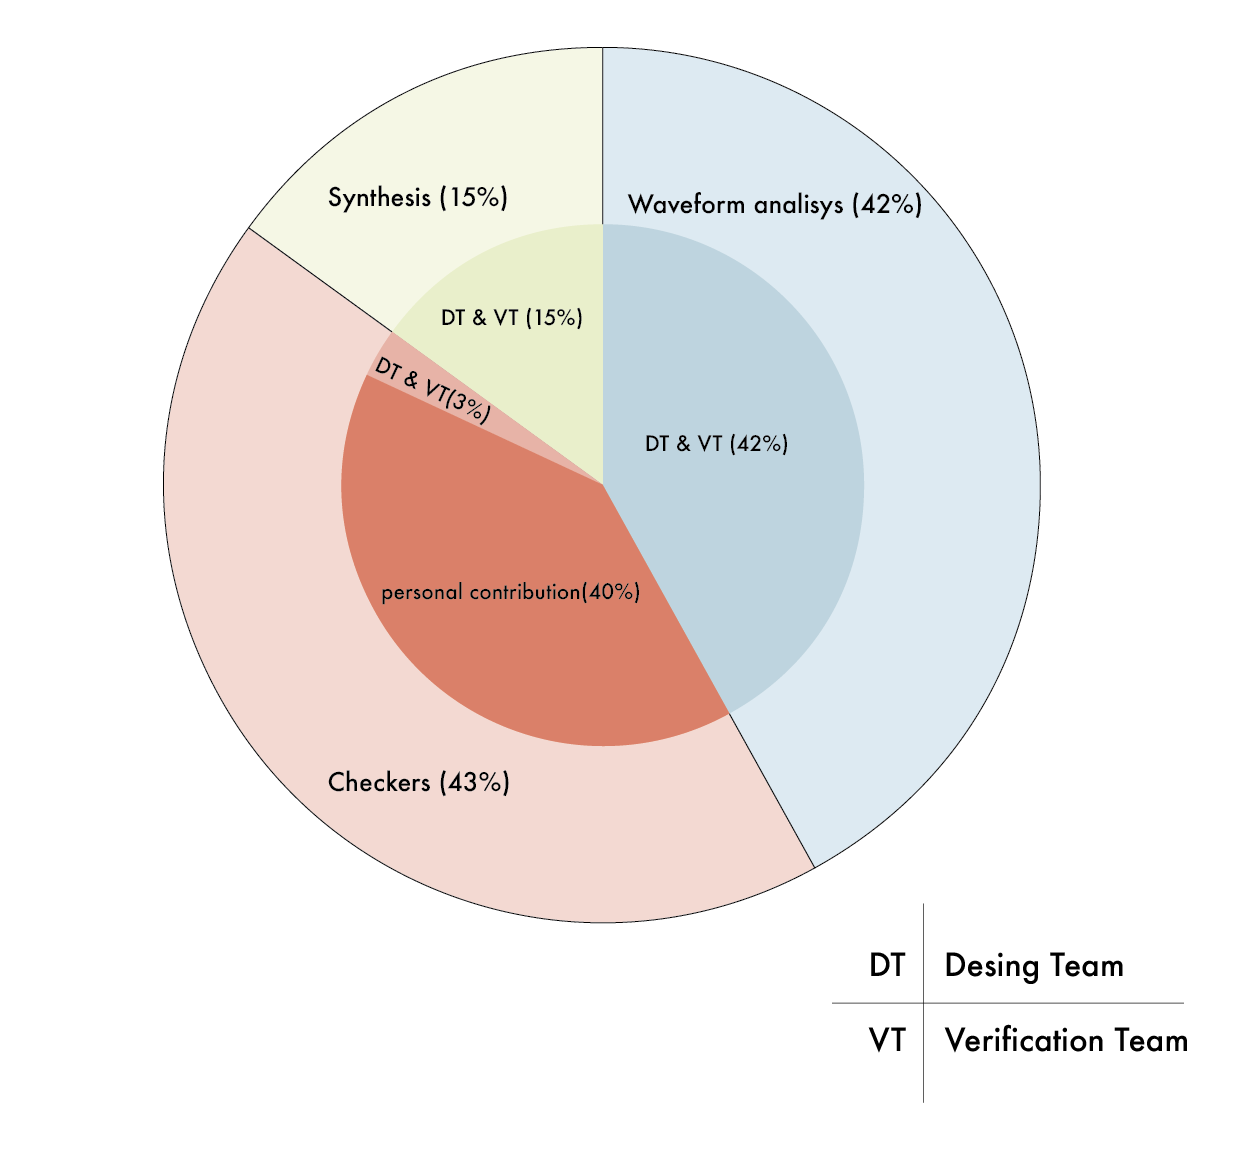
\includegraphics[scale = 0.6]{Chapter_3/img/torta.png}
    \caption{Found bugs}
    \label{torta}
\end{figure}

All the bugs found can be grouped in three categories: \emph{Synthesis}, these are problems related to unconnected wires uninstantiated logic; \emph{Waveform and specifications analysis}, these are all the bugs found simply analyzing the waveform or the specifications, tracing back the error, starting from a wrong result of the VPU; the \emph{Checkers}, in this category there are all the bugs directly found using assertions and assumptions.

As displayed, not all the "checkers" errors were found using the tools created in this work, because some of them were spotted using assertions on the interfaces developed by the Verification Team.

